\section{Kepler Pipeline}

The Kepler Pipeline \cite{2010ApJ...713L..87J} is a data reduction pipeline used for translating the Kepler raw pixel data into possible transiting planet detections. Kepler mission perform photometric observations of carefully selected stars (around 156,000) using its 115 deg$^2$ field of view (FOV) as reviewed in Borucki et el. (2010) \cite{Borucki977}
 and Koch et al. (2010)  \cite{2010ApJ...713L..79K}. The Kepler Mission Science Operations Center (SOC) at NASA Ames Research Center performs major functions on these datasets including calibrate CCD array, download data (light curves) from the spacecraft periodically, remove systematic noise \cite{2012PASP..124.1000S} and perform statistical tests to reject false positives and establish accurate statistical confidence in each detection.

\begin{figure}[!h]
\begin{center}
        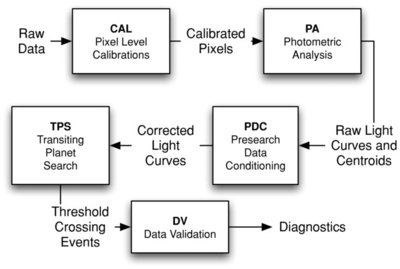
\includegraphics[width=0.5\textheight]{img/kpipeline.jpg}
        \caption{Data flow diagram for the SOC Science Pipeline. Image Credit: The American Astronomical Society}  \label{fig:kpipleline}
\end{center}
\end{figure}

Figure \ref{fig:kpipleline} show the major steps and modules of the pipeline. In particular the last two modules of the pipeline; those that identify as Threshold Crossing Events (TCEs) and their subsequent transit model fiting. TCE is a sequence of significant, periodic, planet transit-like features in the light curve of a target star. Transiting Planet Search module takes systematic error-correlated light curve for a star and seach parameter space for possible transit signatures. This module outputs a TCE or say that does not exists TCE event on the target star. This produce smaller subset of target stars what is given to the Data Validation (DV) module. DV module takes initial TCE and gaps the transit signatures from the light curve and uses the Transiting Planet Search to find additional TCEs on the same target star. This process repeats until it finds all the TCEs on given star. More details on this process explained by Mandel and Agol (2002) \cite{2002ApJ...580L.171M} and Claret and Bloemen (2011) \cite{2011yCat..35290075C}.

TPS algorithm detects transit-like features in light curves by applying noise compensating, wavelet-based matched filtering. TPS characterized the power spectral density (PSD) of the observation noise as a function of time to implement a whitening filter in the wavelet domain. The trial transit pulse is whitened and correlated against the whitened flux time series. Features with correlations above the threshold of 7.1$\sigma$ are flagged as potential threshold crossing events and subjected to additional tests in TPS to guard against false alarms.

Algorithm searches a parameter space with varying transit durations $D$ and produce a Single Event Statistics (SES) time series that is the significance of the detection of the reference transmit pulse centered at that particular time for each $D$

\begin{equation}\label{eq:ses}
	SES(t) = N(t) /\sqrt{D(t)}
\end{equation}

$\sqrt{D(t)}$, is the expected signal to noise ratio of a signal that exactly matches the template pulse and $N(t)$ is the correlated time series.



Multiple Event statistics (MES) is constructed that characterizes a significant detection in a search over varying orbital period $p$ and epochs (phase) $t_0$ by folding $N(n)$ and $D(n)$. MES  $>$ 7.1$\sigma$ may produce a TCE if it also passes additional statistical tests. SES and MES are the basis of some of the attributes used in the training set.


\section{KOI and TCE Attributes }

The Threshold Crossing Events (TCE) catalog contain a sequence of transit-like features in the flux time series of a given target star. These TCE data can download from NASA Exoplanet Archive databases \footnote{\url{http://exoplanetarchive.ipac.caltech.edu/cgi-bin/TblView/nph-tblView?app=ExoTbls&config=q1_q17_dr24_tce}}, and also the detail description of the table fields \footnote{\url{http://exoplanetarchive.ipac.caltech.edu/docs/API_tce_columns.html }} are listed as public data. Kepler Object of Interest (KOI) catalog contains object data including many attributes. The detail attributes are listed on NASA Exoplanet Archive website \footnote{\url{
http://exoplanetarchive.ipac.caltech.edu/docs/API_kepcandidate_columns.html}}, and dataset can be download from the arcive tables \footnote{\url{http://exoplanetarchive.ipac.caltech.edu/cgi-bin/TblView/nph-tblView?app=ExoTbls&config=cumulative}}. All these data cab be download as bulk using data tools available in the archive website.

%\section{Some Important Attributes}
%\label{label:important_attributes}
%There are a large number of attributes available in the KOI and TCE datasets. Out of these attributes, following attributes has significant importance in classification process according to the literature. We will be including these attributes along side with other attributes that will be determined by using Independent Component Analysis.

%\begin{itemize}
%	\item $MES_{max}$/$MES_{min}$
%	\item SNR (for all-transit model fit)
%	\item MES scaled by SES auto-correlation statistics
%	\item $\chi^{2}$ statistics for the all-transits model fit
%	\item Ratio of the planet's semi-major axis to stellar radious
%	\item The proportion of the light curve that was missing during this TCEs transit
%\end{itemize}

\section{TCE Classification Labels}

Each Threshold Crossing Event (TCE) is subject to a vetting process performed by the Kepler TCE Review Team (TCERT). During the triage (Initial) vetting stage, all TCEs are partition into two different sets: Problematic Ligh Curves that has instrumental noise and Kepler Object of Interest. KOI is a TCE that contains convincing transit-like features that do not present obvious evidence that the TCE was generated from non-transiting phenomena such as instrumental noise. These KOIs moves to next level of the vetting process performed by individuals manually inspecting light curves using detection statistics. Any indication they see the signal came from an eclipsing binary star or more complex forms of instrumental noise removed from the list. TCEs that survive this removal process are classified as Planet Candidates (PC).


We can identify three different types of classification labels in the processed dataset: Planetary Candidates (PC), Astrophysical False Positives (AFP) and non-transiting phenomena (NTP). PCs are confirmed as planets, statistically validated as planets or determined to be a planet candidate by the TCERT. AFPs are those TCEs that have been shown to be eclipsing binary stars or have shown evidence that the transiting object being detected is not located around the target tart. NTP are those TCEs that failed the initial vetting process.

%I am planning to use machine learning algorithm (Neural Network) to find a function that maps attributes produced by the Kepler Pipeline for each TCE to a classification label of PC, AFP or NTP. This classification funtion is purely based on the statistical distributions of the attributes for each TCE and the algorithm does not attempt to physically model the process of the planet transit beyond what is already present in the TCE attribute catalogs.


% \todo{Define the Problem we are solving - Classify the TCE catalog is the probme we are trying to solve}
\section{The Problem statement}

Kepler is a single instrument spacecraft that collect most contiguous and long-running photometric time series possible. Kepler observe approximately 170,000 stars simultaneously while it is operating. The fundamental objective of the Kepler mission is to detect a large number of transiting exoplanets. The ultimate goal of the primary mission was a characterize the frequency of exoplanets on diameter, orbital period and host star.  The Manual classification of the findings of Kepler object has proven very time-consuming. The new space-based, transit photometry missions such as K2 \cite{2014PASP..126..398H}, TESS \cite{2014SPIE.9143E..20R}, and PLATO 2.0 \cite{2014ExA....38..249R} also produce a large number of the dataset that demands some level of automation to do the classification. 

Using machine learning classification techniques, we can speed up the process and provide a more continuous rating of planarity candidates. There are various of machine learning classification techniques has been applied to Kepler dataset including random forests, SVM, K-mean clustering \cite{2015ApJ...800...99T, 2015ApJ...806....6M}.  In this project, we are attempting to train a Multilayered Neural Network to identify the potential planetary candidates in the Kepler dataset. 


\section{Solution Statement}

Machine learning techniques contribute a way to automate some step of exoplanet discovery. The TCE vetting process is a tedious and time-consuming (mostly a manual) process. Modern astronomical observational instruments generate a large amount of data within a short period of observational time. These observations may contain such a crucial events that need future follow-up observations using other telescopes (using other wavelengths); hence, processing these time series data and extracting meaningful information is a time sensitive process. Solution to this is to process Kepler data using machine learning algorithms to express the classification while reducing human errors. I am attempting to trained Neural Network to process the TCE catalog to automate the classification process. 
